% Modes
%  draft - drafting mode, esp for todos
%  final - final mode
%
% Other
%  print - do not color links
%
\documentclass[draft,master]{swathesis}

\addbibresource{thesis.bib}

\usepackage{titlepage}
\TitlePageStyle[
subject=master,degree={Master of Science},
]{hpi-swa}

\lstset{language=JavaScript}

\supervisors{
Prof.\,Dr.\,Robert Hirschfeld\and
Bastian Steinert
}

% ABGABEDATUM
% \setdate{2012}{04}{05}
% \date{\datedate}

\author{Lauritz Thamsen}
\location{Potsdam}
\extratitle{\raggedleft Thamsen, \\ Object Versioning for the Lively Kernel\par}
\title{Object Versioning for the Lively Kernel}
% \subtitle{Ein Untertitel ist Optional}

\begin{document}
\frontmatter
\maketitle
%
% abstract.tex
% Abstract / Zusammenfassung
%
\begin{abstract}

% Background
In programming systems such as the Lively Kernel programmers construct applications from objects.
Dedicated tools allow them to manipulate the state and behavior of objects at runtime.
Programmers are encouraged to make changes directly and receive immediate feedback on their actions.

% Problem Statement
When programmers, however, make mistakes in such programming systems, they need to undo the effects of their actions.
Programmers either have to edit objects manually or re-load parts of their applications.
Moreover, changes can spread across many objects.
As a result, recovering previous states is often error-prone and time-consuming.

% Approach
This thesis introduces an approach to object versioning for systems like the Lively Kernel.
Access to previous versions of objects is preserved using \emph{version-aware references}.
These references can be resolved to multiple versions of objects and, thereby, allow re-establishing preserved states of the system.

% Results
We present a design based on proxies and an implementation in JavaScript.
An evaluation shows that the Lively Kernel can run with our proxy-based version-aware references and that preserved system states can be re-established.
The memory overhead of the version-aware references is reasonable.
The execution overhead is not yet practical.
% Conclusion
However, with performance improvements, the solution could be used to provide practical recovery support to programmers.

\end{abstract}




\begin{zusammenfassung}

In Programmiersystemen wie dem Lively Kernel können Programmierer Anwendungen aus Objekten erstellen.
Dabei erlauben dedizierte Werkzeuge den Zustand und das Verhalten von Objekten zur Laufzeit zu verändern.
Programmierer werden ermutigt Änderungen direkt zu machen und erhalten umgehend Feedback.

Wenn Programmierer in solchen Programmiersystemen aber Fehler machen, müssen sie Änderungen rückgängig machen.
Dazu müssen sie entweder Objekte manuell bearbeiten oder Teile ihrer Anwendungen neu laden.
Die gemachten Änderungen können dabei über viele Objekte verteilt sein.
Vorherige Zustände wiederherzustellen ist deshalb häufig schwierig und zeitaufwendig.

Diese Arbeit stellt einen Ansatz für die Versionierung von Objekten in Systemen wie dem Lively Kernel vor.
Der Ansatz basiert auf \emph{Versions-bewussten-Referenzen}.
Diese können zu mehreren Versionen von Objekten aufgelöst werden und erlauben so vorherige Systemzustände wiederherzustellen.

Für den Ansatz beschreibt diese Arbeit eine auf Proxys basierenden Implementierung in JavaScript.
Eine Evaluierung davon zeigt, dass die Implementierung es erlaubt Systemzustände des Lively Kernels zu erhalten und wiederherzustellen.
Der zusätzlich nötige Arbeitsspeicher für die Versions-bewussten-Referenzen ist dabei vertretbar, während die Programmausführung erheblich verlangsamt wird.\\
Mit Verbesserungen könnte die Lösung allerdings benutzt werden, um Entwickler mit praktikablen Wiederherstellungs-Werkzeugen zu unterstützen.

\end{zusammenfassung}

%%% Local Variables:
%%% mode: latex
%%% End:

% \begingroup
\let\raggedsection\centering

\chapter*{Acknowledgments} \label{cha:acknowledgments}
\endgroup

\begin{quotation}
  \noindent I am grateful to my supervisors Bastian Steinert and Professor Robert Hirschfeld for their guidance and support. 
\end{quotation}

\begin{quotation}
  \noindent I am thankful to Jens Lincke, Marcel Taeumel, Tobias Pape, Tim Felgentreff, Michael Perscheid, Stephanie Platz, Carl Friedrich Bolz, Robert Krahn, and Dan Ingalls for fruitful discussions and valuable input.
\end{quotation}

\begin{quotation}
  \noindent I thank Oliver Buck for his comments on drafts of this thesis.
\end{quotation}
\tableofcontents
\listoffigures
% \listoftables
% \lstlistoflistings
% \listofacronyms
\mainmatter

% I. Background and context (problem area and motivation) 
% II. However (problem description)
% III. So what? (problem dimension) 
% IV. Deficiencies with previous approaches
% IV. Solution

\chapter{Introduction} \label{chapter:INTRODUCTION}

% Background
Programming systems such as Squeak/Smalltalk~\cite{Ingalls1997Squeak,GoldbergRobson83} and REPLs for LISP or Python allow to adapt and develop programs while those run.
Changes to programs in such environments are effective immediately and programmers can often see or test right away what differences their actions make.
Thus, these systems provide immediate feedback to programmers.
A subset of such systems, which includes, for example, Self~\cite{Ungar1987SPS,Ungar2007SEL} and the Lively Kernel~\cite{Ingalls2008LKS,Krahn2009LWD}, are those built around prototype-based object-oriented languages, in which programmers create applications using objects and without having to define classes first.
In these systems, programmers can inspect and change the state of objects at runtime and can add and modify object-specific behavior.
The results of such development are actual objects, not source code that only abstractly describes potential objects.

The Lively Kernel was designed to support this kind of development and focuses, hereby, on graphical objects.
For this, the Lively Kernel provides tools to directly manipulate the style, the composition, and the scripts of graphical objects.
For example, programmers can change positions and the composition directly using the mouse.
They can edit and try methods directly in the context of graphical objects, or use temporary workspaces to manipulate one or many objects programmatically.
For example, to add new functionality to a graphical application, a programmer might copy an existing button object and then directly modify the newly button object: move the new button to a sensible position, resize it slightly, set a new label, and add a script to be executed on each mouse click.
The programmer makes all these changes directly to one button object and, for example, how the button fits into the application's interface is visible at all time, while clicking the button allows to directly test its functionality.
This way, the Lively Kernel often allows for fast feedback, especially during the development of graphical applications.

% Problem
Changes programmers make to objects---either using specific tools or through executing code---can, however, also turn out not to be improvements and still permanently affect objects.
Programmers can, for example, accidentally change the positions, accidentally connect the wrong objects when manipulating applications with mouse interactions, or make a mistake in a workspace code snippet that then manipulates many objects differently than intented.
Similarly, programmers might learn in hindsight that making a promising change to an object's scripts actually introduced an error or impacts the application's performance.
Less accidental but still problematic, they might try a couple of different alternatives as, for example, different color schemes and graphical layouts, only to realize later that an earlier state was most appealing and should thus be re-established.
Other potentially inappropriate changes might be introduced when code is evaluated to understand or test behavior, not to permanently change state.

% So what?
When changes, however, do turn out to be innapropriate, programmers often need to undo them manually or need to have prepared for potential negative outcomes in advance.
That is, the Lively Kernel does not provide an undo for changes to objects, which is especially at odds with the Lively Kernel's support for trying ideas right away: Developers are able to make changes directly and frequently receive immediate feedback, but do not get support when changes turn out to be inappropriate.
So, when programmers want to recover a previous development state, they often need to manually reset the state to how it previously was---often using the same tools the changes were initially made with and potentially involving multiple properties of multiple objects changed by multiple developer actions.

The Lively Kernel provides tools to commit and load versions of objects.
In case such commits exist, programmers can load earlier versions of objects to re-establish previous states.
Nevertheless, depending on how far such a commited version is from the actually desired state, manual changes might still be necessary.
Thus, to keep the effort required to re-establish \emph{any} previous state low, programmers would need to commit many versions.
However, these commits would partly be made only to preserve intermediate development states, not to share and document work results but to protect against changes that unexpectedly turn out to be mistakes.
The commits would further also require significant effort, especially when the preserved versions should be usable and documented, requiring states to be either tested and augmented with useful descriptions right away, or else requiring developers to actively clean up repository histories regularly.\\
\emph{In summary}, recovering previous states of objects in the Lively Kernel is currently a significant effort for programmers as they either have to manually re-set changed state or to take significant precautionary actions.\\

A typical approach to implementing multi-level undo for the changes to state of applications is the Command pattern~\cite{GammaHelmJohnsonVlissides95}.
The command pattern packages changes into actions.
It can then record actions and, when each action has been provided with an undo counterpart, subsequentely undo them.
This, however, requires developers to implement specific undos for all possible actions, which even for just the existing tools to manipulate objects in the Lively Kernel would result in a rather comprehensive implementation and which would of course also require developers to accompany each newly implemented manipulation tool with undos.  
Further, this approach is entirely unpractical for undoing the effects of evaluating arbitrary code snippets as, for example, regularly done in the Lively Kernel's workspaces.

Worlds~\cite{Warth2011Wor} is a recent and more generic approach using a language construct for controlling the scope of side-effects from arbitrary code.
It allows to capture the side-effects of statements into different \emph{worlds}.
These worlds can be used to run code with particular sets of changes being effective.
Developers could, thus, execute all their actions in separate worlds and discard those worlds when necessary to return to previous ones.
Worlds as such, though, would require developers to explicitly create as well as potentially merge or discard worlds, and, therefore, still needs the programmer to explicitly take precautionary actions, similar to version control systems.
In addition, the implementation of Worlds for and in JavaScript is not yet practical as it, for example, currently prevents garbage collection.

In contrast to these approaches, CoExist~\cite{Steinert2012COE,Steinert2014EVA} provides automatic recovery support, without requiring developers to take any precautionary actions beforehand.
For this, CoExist automatically records versions for every change and, thereby, provides a fine-grained history of intermediate development states.
To each preserved version programmers can also see diff views, screenshots, and test results.
Programmers can review the changes chronological, examine the impact each change had, and re-establish previous development states again.
However, CoExist currently recognizes only changes made to the source code of classes and does not preserve the state of objects.

% Solution
This thesis proposes to version the entire state of programming runtimes as basis for automatic recovery support in systems like the Lively Kernel.
In particular, this thesis introduces an approach to preserving and managing versions of all objects, which make up different runtime states, using alternative, \emph{version-aware} references.
Version-aware references are alternative references in that they can refer to multiple versions of objects, but always resolve transparently to one particular version among those.
Versions of objects are preserved together, so that the version-aware references can be resolved transitively to state as it was at a particular moment.
For this to be practical, versions of objects can be kept in application memory and the state of all objects can be preserved incrementally, on writes and only for objects that actually change.
Similarly, to which versions the version-aware references resolve can also be changed without significantly interrupting program execution:
The version-aware references can decide dynamically to which versions they resolve instead of being hard-wired to specific versions.

We implemented version-aware references for the Lively Kernel in JavaScript, on the level of the language using proxies and source transformations and, thus, without requiring adaptions to established execution engines.
Proxies implement version-aware references.
They stand in for references: conventional references point to them and they delegate all object access--all kinds of read and write operations--transparently to one particular version of the object they can stand in for.
A combination of proxy behavior and source transformation then allows to introduce and use these proxies consistently for all objects, in order to version the entire runtime state as is necessary for completely generic recovery support.

We designed and implemented this approach to object versioning for the Lively Kernel with the intention to provide CoExist-like recovery support, including continuous versioning, in the future.
Therefore, this approach supports fine-grained histories of development states---many, but still particular versions of the entire runtime that can correspond to developer actions and can be re-established quickly.
It also allows to easily enhance preserved development states with further information as, for example, test results, screenshots, and diffs.
That is, in the future, we want to build upon the presented solution and support developers in efficiently recovering state from continuously preserved, fine-grained histories of development sessions.

\section{Contributions}

The goal of this work is to provide a basis for automatic recovery support for systems like the Lively Kernel.
To that effect, the main contributions of this thesis are the following:

\begin{itemize}
    \item An approach to object versioning for systems like the Lively Kernel based on alternative, version-aware references that transparently delegate to one of multiple versions of an object (Section~\ref{sec:APPROACH:1}).
    \item A concrete, language-level solution that provides the proposed version-aware references through proxies and source transformations for the Lively Kernel (Section~\ref{sec:APPROACH:2}).
    \item An implementation of the concrete solution in JavaScript that can be used to effectively preserve and re-establish development states of the Lively Kernel (Section~\ref{chapter:IMPLEMENTATION}).
\end{itemize}


\section{Thesis Structure}

The remainder of this thesis is organized as follows. 
Chapter~\ref{chapter:BACKGROUND} describes prototype-based programming systems, CoExist, and the Lively Kernel.
Chapter~\ref{chapter:MOTIVATION} illustrates how developers directly manipulate objects in the Lively Kernel and exemplifies characteristic recovery needs associated with this kind of development.
Chapter~\ref{chapter:APPROACH} introduces our approach to object versioning and describes how proxies can be used for concrete solutions.
Chapter~\ref{chapter:IMPLEMENTATION} presents our implementation for the Lively Kernel, which Chapter~\ref{chapter:EVALUATION} then evaluates in terms of functionality and practicability.
Chapter~\ref{chapter:RELATED_WORK} compares our solution to related work.
Chapter~\ref{chapter:FUTURE_WORK} presents future work, while Chapter~\ref{chapter:CONCLUSION} concludes this thesis.

\chapter{Background} \label{chapter:BACKGROUND}

Our goal is to provide generic recovery support for prototype-based programming systems and we implemented our approach for the Lively Kernel, a particular example of such a system.
Prototype-based programming systems use objects directly as building blocks for applications without requiring more abstract entities like classes.
The Lively Kernel is a prototype-based, self-supporting, and web-based programming system with tools to directly manipulate graphical objects.

Our approach and the implementation are intented to provide similar automatic recovery support to programmers as CoExist does.
CoExist applies continuous versioning to provide programmers with access to a fine-grained history of development states without requiring them to take any explicit precautionary actions themselves.


\section{Prototype-based Programming}

Prototype-based programming is object-oriented programming in which applications are constructed using only objects, without classes.
Examples for programming languages or systems that implement prototype-based programming are Self, JavaScript, and Kevo~\cite{Taivalsaari1992Kevo}.
Self and JavaScript incorporate prototypical inheritance.
They allow objects to inherit state and behavior directly from other objects: an object has a prototype to which it delegates when looking up a property in the object itself yields no results.
Kevo, in constrast, does not provide this kind of delegation, but instead allows to make full copies of objects, so objects in Kevo do not share behavior or state.
Programmers can create new objects with initially the same state and behavior as existing ones, but all objects remain self-contained.
That is, in Kevo, changing an object only changes that particular object and a particular object can only be changed by directly changing it, not by changing any other artifact.
To adapt many objects at once Kevo, programmers can only use so-called \emph{module operations} that are evaluated on a group of objects. 
Despite this difference in whether properties can be shared among objects and how to then affect families of objects, prototype-based programming always allows to build programs from particular objects, in contrast to the class-based style of object-oriented programming, in which programs are defined in abstract descriptions of structure and behavior.
In particular, the parts of a program are objects with particular state, specific examples rather than general categories.

There are different advantages associated with this kind of programming:
\begin{itemize}
    \item \cite{Taivalsaari1996CVP} and \cite{Ungar1987SPS} argue that it might be easier for programmers to understand concrete examples compared to abstract classes. A concrete example provides particular values for its state and, in case of objects with a visual appearance, can be actually looked at.
    \item \cite{Ungar1987SPS} and \cite{Borning1986CVP} describe how prototype-based programming makes it easier to introduce one-of-a-kind objects with their own structure or behavior.
    \item \cite{Borning1986CVP} and \cite{Maloney1995Mor} make the point that especially editing visual objects can be more concrete with prototypes. Instead of writing code to define the appearance of objects, programmers can manipulate particular visual objects directly. Programmers could, for example, use the mouse to manipulate properties like the size, position, and style or to combine multiple basic elements into one composition. This way, programmers always see intermediate states and do not only receive feedback on explicit test runs in-between edit-compile-load cycles or run/edit distinctions. 
\end{itemize}

Similarly to the previous examples, many end-user programming systems, including Scratch\cite{Maloney2010SPL}, Etoys~\cite{Kay2005Etoys}, and Fabrik~\cite{Ingalls1988FVP}, enable users to express their programs through particular objects, all with graphical representations and tools to directly manipulate those.
In addition, programmers manipulate objects at runtime both in these end-user programming systems and in many general-purpose prototype-based programming systems like the Lively Kernel, Self, and Kevo.
Further, most of these systems also provide tools for manipulating graphical objects directly, where graphical objects range from simple objects like primitive shapes over interactive widgets to applications like presentation software or programming tools.
In general, programming at runtime, prototype-based programming, and direct manipulation of graphical objects seem properties that suit each.


\section{The Lively Kernel}

The Lively Kernel is a browser-based programming system in the tradition of both Smalltalk and Self.
Development in the Lively Kernel happens at runtime and it incorporates tools and techniques to be completely self-sufficient.
Thus, pogrammers can create versions of the Lively Kernel with the Lively Kernel.

The Lively Kernel is based in the JavaScript programming language.
Therefore, the system and applications are expressed in a prototype-based object-oriented language that also provides prototypical inheritance.
At the same time, the Lively Kernel also provides a class system for JavaScript and considerable parts of the system itself are expressed using this class system.
One of these parts expressed through classes is an implementation of Morphic~\cite{Maloney1995Mor}, a framework for developing graphical applications.
Programmers can alter graphical objects of this framework, which are called \emph{Morphs}, using direct manipulation and through a number of dedicated tools.
While the framework and other parts of the core system are expressed using classes, these morphs are an example of objects that are often edited directly and not through adapting existing or creating new classes.
Though each morph does have a class, it can have not only its own state, but object-specific behavior---thus the Lively Kernel effectively mixes the prototype-based and the class-based flavors of object-oriented programming.

\begin{figure}[h]
    \centering
    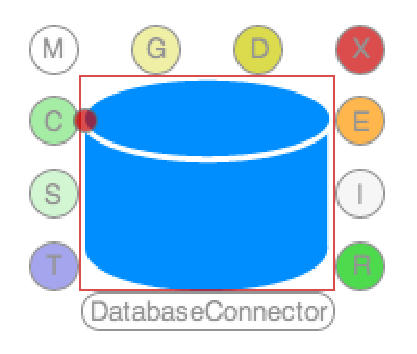
\includegraphics[width=0.3\textwidth]{figures/2_background/1_halos.pdf}
    \caption{The halo buttons of a simple morph.}
    \label{fig:Halos}
\end{figure}

Programmers can change the position of morphs by dragging and the composition by an alternative dragging, which is called \emph{grabbing}.
That is, the composition of morphs is also part of Morphic and a morph can have submorphs.
This way, morphs are not limited to to be basic shapes or simple widgets, but can be entire user interfaces of arbitrary applications.
The Lively Kernel provides a set of manipulation tools, called \emph{Halos}, as shown in Figure~\ref{fig:Halos}, that developers can bring up directly at morphs.
The different halo buttons allow, for example, to resize~\textcircled{R}, rotate~\textcircled{T}, and copy~\textcircled{C} morphs.
The copy operation does not establish a prototypical inheritance relationship between the copy and the original, but instead copies the entire state, including of which class the copy is an instance.
Other halo buttons open specific tools, which are shown in Figure~\ref{fig:LivelyTools} to further manipulate the morphs:

\begin{enumerate}
    \item The \emph{Inspector}~\textcircled{1} presents all the values that make up a morph's state. It also has a small code pane at the bottom, which is intended to be used to manipulate the state programmatically.
    \item The \emph{Style Editor}~\textcircled{2} allows to manipulate certain aspects of a morph's visual appearance. Programmers can use it to, for example, change a morphs color, border width, or the layout of its submorphs.
    \item The \emph{Object Editor}~\textcircled{3} is a tool dedicated to the object-specific behavior of morphs, which are called \emph{scripts} in the Lively Kernel. It shows all scripts of a particular morph, but also can add and adapt scripts.
\end{enumerate}

\todo{smaller numbers in the Figure..}

\begin{figure}[h]
    \centering
    \includegraphics[width=\textwidth]{figures/2_background/2_LivelyTools.pdf}
    \caption{The Lively Kernel's tools to manipulate properties of morphs, from left to right: the Inspector, the Style Editor, and the Object Editor.}
    \label{fig:LivelyTools}
\end{figure}

\begin{figure}[h]
    \centering
    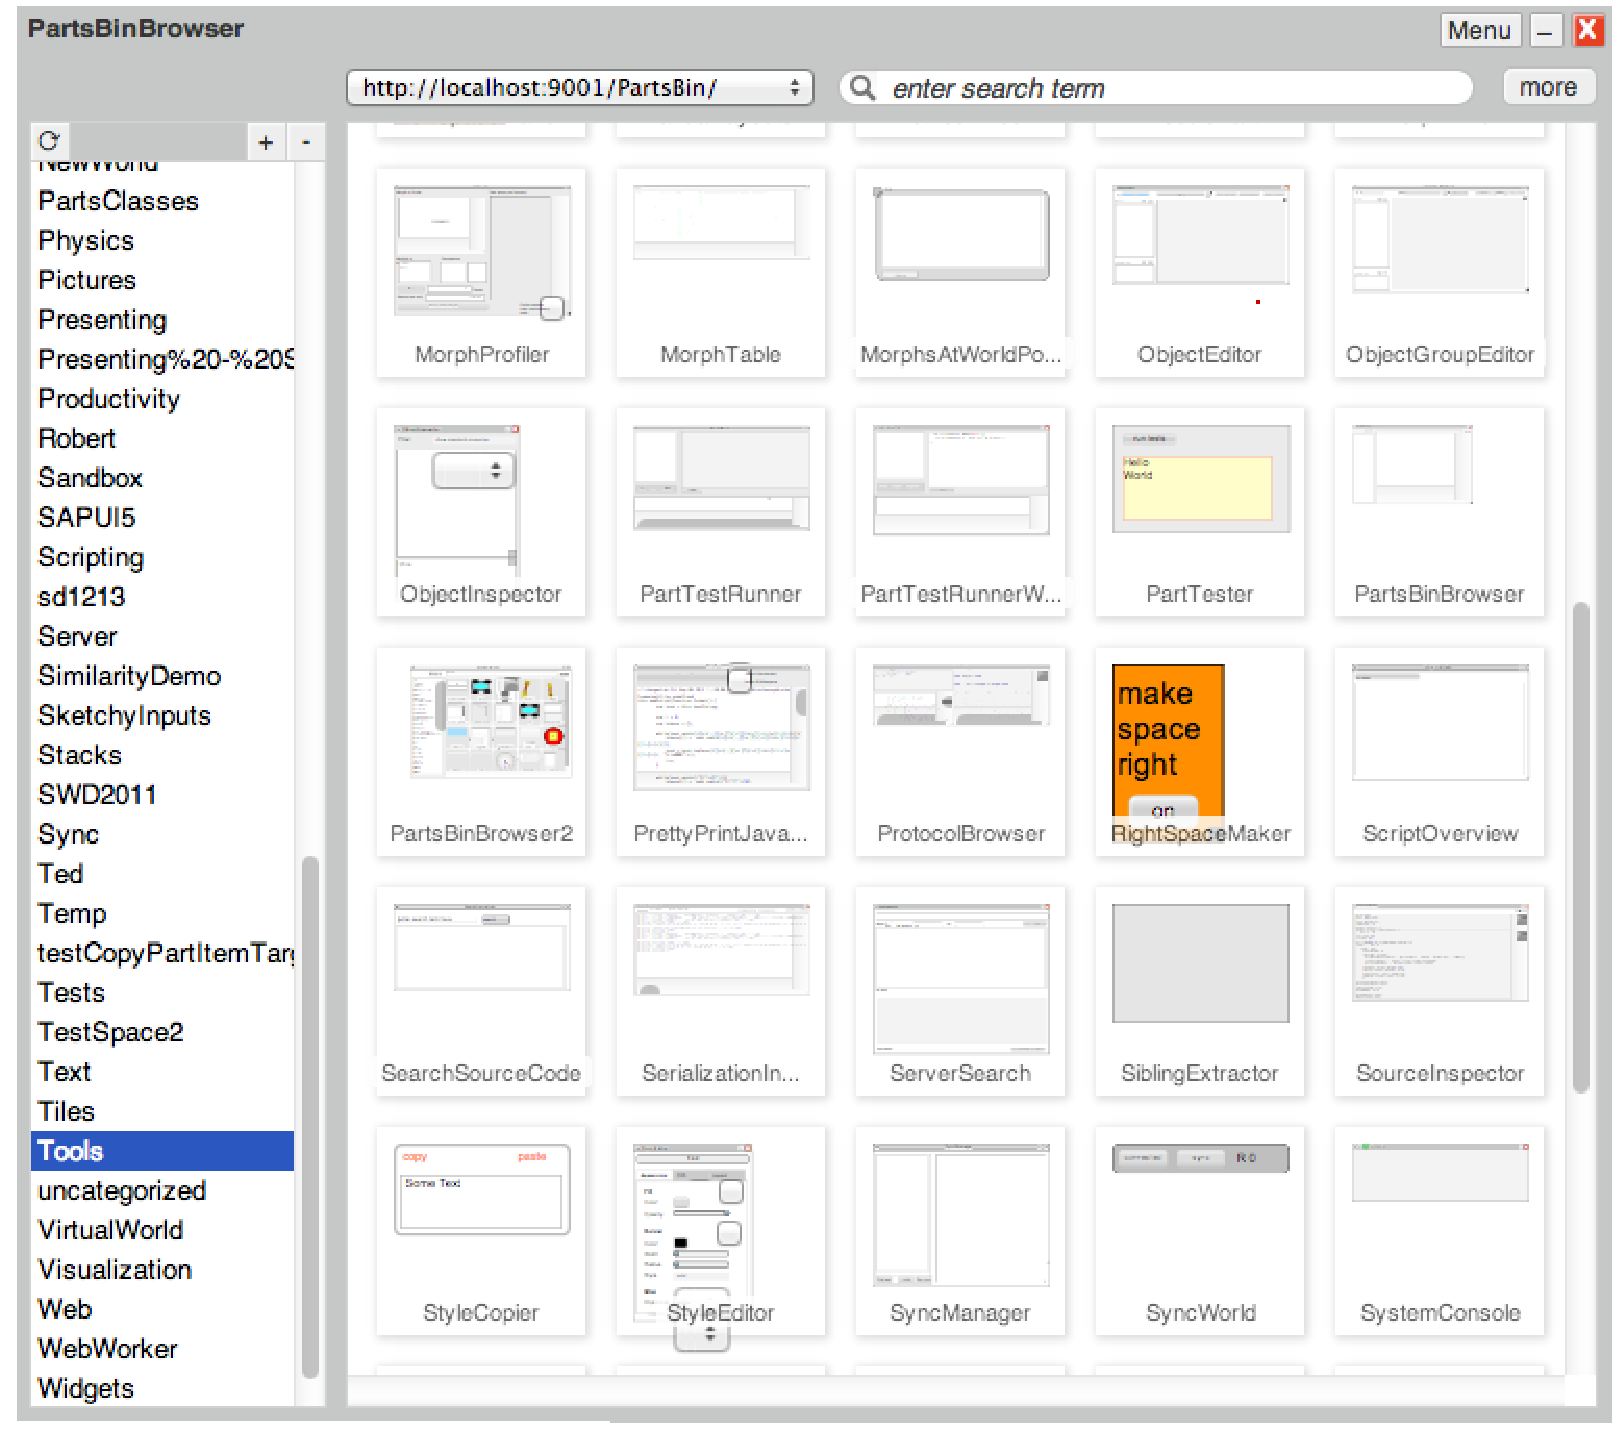
\includegraphics[width=0.7\textwidth]{figures/2_background/3_partsBin.pdf}
    \caption{The Lively Kernel's Parts Bin opened on the \emph{Tools} category.}
    \label{fig:PartsBin}
\end{figure}

Another tool related to morphs, though not available from a halo button, is the Lively Kernel's \emph{Parts Bin}~\cite{Lincke2012LPC}, an object repository to commit and load specific versions of morphs.
Morphs saved to the Parts Bin are called \emph{parts} to emphasize the ability to reuse any one of the morphic applications stored in the Parts Bin for other applications.
Figure~\ref{fig:PartsBin} shows the Parts Bin and, in particular, a group of tools that the Parts Bin contains, which includes both the Style Editor and the Object Editor.
Both these tools are examples for graphical applications developed from available parts, with their logic expressed in scripts, and available to users through the Parts Bin.


\section{CoExist}

The CoExist system\footnote{\url{http://www.bastiansteinert.org/coexist.html}, accessed February 28, 2014} and approach supports programmers through automatic and continuous versioning.
CoExist preserves each indermediate development state with its respective source code and associated runtime information.
The states are recorded as separate version in their original order and along with change summaries, associated test results, and screenshots of the development environment.
Programmers can review their development sessions, inspect the impact each individual change had on test cases, and recover previous development states.
They can completely withdraw withdraw changes or only re-visit a previous state to recover partial information as, for example, the source code for a specific method.

\begin{figure}[h]
    \centering
    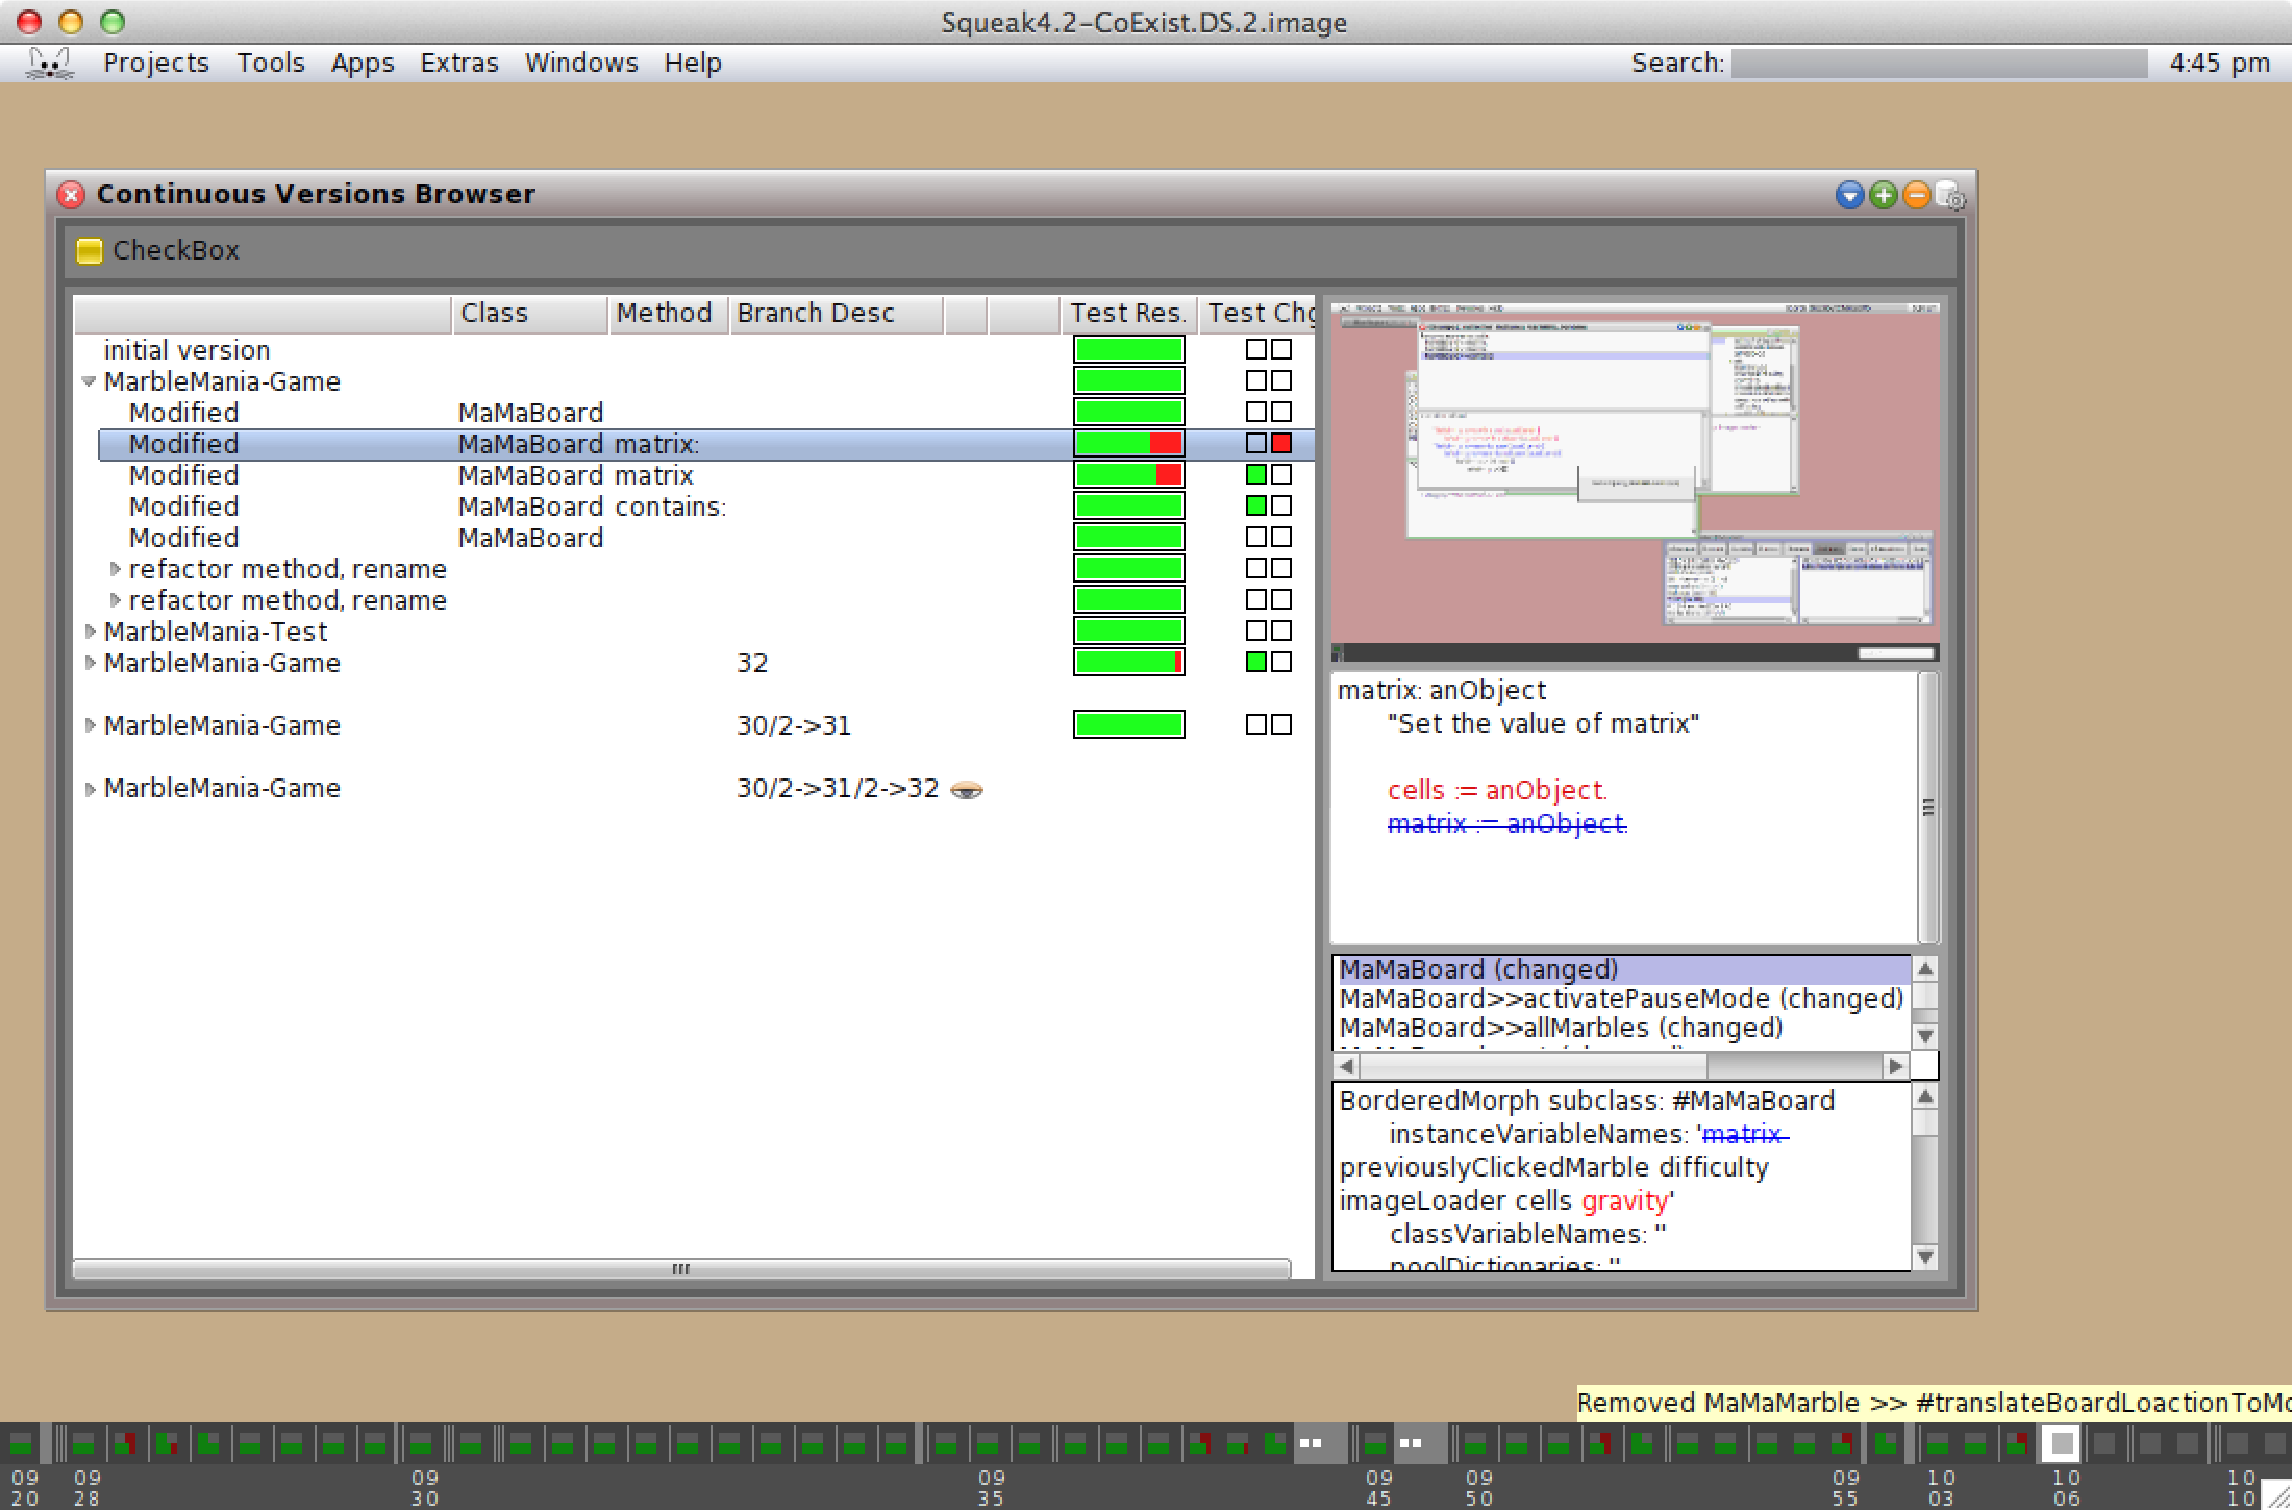
\includegraphics[width=\textwidth]{figures/2_background/4_coexistTools.pdf}
    \caption{CoExist's tools to manage the preserved development states: a timeline and a Version Browser.}
    \label{fig:CoExist}
\end{figure}

CoExist provides tools to help programmers benefit from the preserved development histories, shown in Figure~\ref{fig:CoExist}.
A timeline tool at the bottom of the development environment presents each intermediate version through a small rectangle that indicates the impact on test cases: the bottom of the rectangle shows how many test cases passed and failed absolutely, while the top half highlights only test results affected by the changes of this particular version.
Hovering above such a version rectangle indicates what exactly changed in terms of methods and classes.
Clicking a version provides access to its source code and more information on test results, but also allows to re-establish the version.
Besides this timeline of versions, a Version Browser tool shows changes in a different structure, also chronological, but separately for different source code modules.
It presents the same information on test cases, but in addition also offers diffs and how the development environment appeared visually in each version through providing screenshots.
The two tools support programmers in re-tracing their steps, understanding the impact of their actions, and in recovering information from previous development states.

CoExist is intented to reduce the effort that programmers usually put into recovery, either into actual compensational actions or into precautionary actions, and, thereby, also to help programmers to overcome any aversions to try new ideas.
To re-establish a previous development state---because of, for example, unintentionally introduced errors, decreased performance, or harmed program design---programmers can manually repair improperly changed code or load a previously commited version of the sources.
Programmers can preserve specific versions to be able to easily withdraw changes, and, thereby, reduce the cost of recovery by anticipating recovery needs beforehand.
However, preserving versions manually is also an effort and especially so when revision histories are expected to be well-documented and immediately useful.
For that, programmers need to assemble changes to meaningful increments, test these, and write helpful commit messages.
Testing each one directly is also advocated as it can help to find introduced problems directly intead of later analyzing long lists of changes that all could potentially have introduced a problem.
With CoExist, developers do not have to take these explicit precautionary actions, but still have access to a fine-grained history of development states and even test results for each individual state.
Instead of worrying about negative consequences when trying ideas, programmers can focus on their actual programming tasks and rely on CoExist to help in case any action unexpectedly needs to be undone.

% \todo{Structured: not just like auto-save (google docs), but structured: associated with particular actions and the static structure of programs... class>>method (add/delete/modify).. and also cross-document}

% % sometimes easier to make the changes and experience the results than to anticipate the changes beforehand...)

% have to remember to make commits +  
% commits take some effort: combining changes into meaningful increments, making sure the current version passes test cases, where test cases also take time, writing helpful commit messages
% for this reason, not a commit for every single change, but deciding when to commit, assessing the risks of changes and planning changes to a point where grouping changes into consistent steps, which each should be commited separately, is also time-consuming and error-prone

\chapter{Approach} \label{sec:APPROACH}

\todo{better title?}



\section{Idea: Object Versioning}

version-aware references: references that know multiple versions of the same object and choose a particular version of it at runtime when accessed 

versions of the object corresponding to versions of the runtime, which may get created explicitly by the programmer, but also could be created with manipulating user interactions (saving source code, evaluating do-its, directly manipulating graphical attributes and composition, other events). so, for a given version of the runtime, there are versions of the object. setting a version of the runtime then determines which version of an object is used when the reference to that object gets resolved.

versioning the programming runtime, while side effects to state of other programs, or server processes, or databases cannot be reversed with this approach 






% \section{3.X why an implementation solely in javascript}
% 
% implementation in the JavaScript language, without changing the virtual machine: use objects as references, make sure those objects are used everywhere..
% 
% * proxies to implement version-aware references
% * source transformations and proxy behavior to use version-aware references consistently
% * global versions and proxy behavior to have particular versions of the runtime





\section{Proxies as Version-aware References}

implementation in javascript, so there are only actual references in JavaScript, but we can use objects that represent references that know multiple versions of objects.

but as resolving a version-aware reference should transparently result in a particular version of the object, these objects need to delegate transparently to that particular version.
therefore, we use proxy objects for version-aware references, in particular the ECMAScript 6 Direct Proxies.

also we let the proxy objects hold all versions of an object instead of, for example, using object tables, so that when no object holds the version-aware reference any longer, the reference object with all versions of the actual object get garbage collected.



\section{Version-aware References Instead of References}

use version-aware references consistently:
for all references between two objects use version-aware references instead. that is, all usual references need to become references to a proxy objects, which then reference one or multiple versions of the actual object.

given that proxy references are returned as such when reading object properties and variables, it is only necessary to immediately wrap objects when they are created to use proxy references consistently for the system. so, we return version-aware references / proxies instead of the usual references for all new objects that are created.

ways to create new objects in javascript: literals, constructor, specific built-in functions (Object.create.. eval..)

literals can be rewritten to be wrapped into proxies immediately. constructors are functions, which should already be proxied so that proxy behavior can be specified to return proxies for new instances, while specific built-in functions can be patched globally or rewritten for source to also return proxies.



\section{Versions of The Runtime}

particular versions of the runtime

global version data structure for the runtime, runtime versions may have predecessors and may have successors, versions of objects get chosen using the current global version of the runtime

not necessarily necessary to copy each object for each version, but can be done on writes. further, not necessarily necessary to copy objects completely, but diffs or even delegation between diffs in a prototypical manner can be implemented

\chapter{Implementation with Direct Proxies} \label{sec:IMPLEMENTATION}

\todo{add a link to a published github commit}

% \section{3.X why an implementation solely in javascript}
% 
% implementation in the JavaScript language, without changing the virtual machine: use objects as references, make sure those objects are used everywhere..
% 
% * proxies to implement version-aware references
% * source transformations and proxy behavior to use version-aware references consistently
% * global versions and proxy behavior to have particular versions of the runtime

\section{Using ECMAScript 6 Direct Proxies}

% \begin{itemize}
%     \item ECMAScript 6 Direct Proxies\footnote{\url{http://wiki.ecmascript.org/doku.php?id=harmony:direct_proxies},\goodbreak accessed February 3rd, 2014}: proxy handler object, traps; ES 6 in DRAFT ~\cite{ECMA2014ES6}, deprecated Harmony Proxy proposal implemented in current chromes, but 
%     \item proxies for mutable JavaScript objects: objects, arrays, functions
%     \item the proxy handlers really hold references to copies of the same object in a dictionary (version name -> object version)
%     \item delegation to a particular version at runtime using a version of the target object according to some global version of the runtime..
%     \item identity of proxyFor(obj) === proxyFor(obj), ProxyTable (weak-key map, objects -> to their proxies)
% \end{itemize}



proxy implementation limitations: 
\begin{itemize}
    \item proxies as prototypes (relation can’t be changed.. traps of proto fire when inheriting object is accessed.. problem is Chrome and only the proto case...)... protoProxy property on objects..
    \item no instanceof trap, Object.instanceOf source transformation 
    \item [native code] boundary / primitive functions and objects: setting properties / calling functions leads to errors or has absolutely no effect: part 1: traps (sep-trap: onreadystatechange, apply-trap: any DOM function.., Array.prototype.concat, aWorker.postMessage.. multi-level unwrapping for args object, aFunc.apply or aFunc.call).
part 2: patches: Object.isRegExp, ‘some string’.match (done by patching String.prototype.match)
\end{itemize}


\begin{itemize}
    \item DOM redrawing on undo / redo: DOM is out of versioning scope, doesn’t use version-aware references, has to be changed / redrawn on undo/redo explicitly
\end{itemize}




\section{Returning Proxies For New Objects}

goal: all references to newly created objects need to be version-aware references, i.e. references to proxies instead of references to the (initial version of the) target. 

we rewrite instead of patching them globally, because that's not possibly for all built-in objects.
also, our implementation is itself in javascript and, therefore, uses built-in data types, too, which should not be proxied.
for this reasons, we transform the sources of modules loaded after our versioning implementation.

\begin{itemize}
    \item value of literal expressions: source transformations (objects, arrays, function expressions), examples.. function declarations and hoisting, literal accessor functions in object literals
    \item return value of custom constructors: construct-trap (..code for the construct / apply traps of the proxies..)
    \item return value of specific built-in functions and constructors: source transformations (only in the lexical scope of some particular modules, e.g. not for our implementation)
\end{itemize}

[what about all other source transformations..??]

% \begin{itemize}
%     \item why UglifyJS: fast, complete, testing alternative grammar rules during parsing is not implemented using execeptions, provides source maps (all in contrast to OMeta)
% \end{itemize}



\section{Providing Simple Global Versions for Undo and Redo}

JS execution: single-threaded, cooperative scheduling 

\begin{itemize}
    \item global versions, linear versioning, data structure is an version object with a predecessor and a successor
    \item copy-on-write for versions of objects (set-trap, apply-trap for some array methods)
\end{itemize}


\begin{itemize}
    \item source transformations enabled right after the object versioning code, i.e. the implementation of the proxies and the source transformation, which are both themselves javascript code, gets loaded. by patching the eval that is used for evaluated modules that get loaded with an eval(transformSource.. so modules aren’t versioned, but classes / layers / traits are.. e.g. a class is versioned, so in different versions there might be different class-side state... so, for example, modules are currently in our implementation the roots of the version-aware reference graphs that prevent garbage collection, 
\end{itemize}


\begin{itemize}
    \item undo / redo implementation, example situation
    \item redraw of the world as DOM objects / DOM relations are not part of the object versioning in JavaScript
\end{itemize}






\section{Limitations of the Implementation}


% \subsection{Limitations for Concurrent JavaScript Functions}


single-threaded and cooperative scheduling, but setTimeout / setInterval... stop asynchronous actions from following versions when undoing... source transformations, which scripts belongs to which version


% \subsection{Limitations in the Execution Environment}

\begin{itemize}
    \item only works in recent Chromes, with experimental JavaScript... ECMAScript 6 Direct Proxies not yet fully implemented, not yet stable.. shim library\footnote{\url{http://github.com/tvcutsem/harmony-reflect},\goodbreak accessed February 3, 2014, at version 0.0.11}..
.. own adaptions to the shim library, to bridge the gap between the current version of the shim and information from the Spec draft (pass null for the target of a proxy)... fully virtual objects vs. consistency checks.. adapted library to fit spec draft (pass null as target of a fully virtual object, then no trap-return-value-consistency-with-target checks)
\end{itemize}
    


\begin{itemize}
    \item debugging: interference with Chrome's developer tools, which don’t handle proxies well (hovering, labels, stepping into)
\end{itemize}


% \subsection{Usability: Impact on Debugging}

\begin{itemize}
    \item adds lots of ‘low-level’ frames, dev tools don’t handle proxies well (hovering, labels, stepping into), but we have at least source maps, so developers can debug the original code and not the result of our source transformation
\end{itemize}


Besides impacting code execution, the current implementation of object versioning for Lively also  with certain programming tasks.
Though the version-aware references should be transparent to programmers, in the current proxy-based implementation proxies show during debugging.
However, the developer tools show the original source code, despite the implementation's transformations of the sources.

\chapter{Discussion} \label{sec:DISCUSSION}

We tested the implementation with two JavaScript benchmark suites and our target programming system, the Lively Kernel.
The proxies, which implement version-aware references, behave like the respective versions of objects in all situations exhibited.
The linear global runtime versions allows to re-establish previous development states in Lively.
That is, all references to relevant objects appear to be version-aware references in the tested situations.

The memory overhead of our implementation appears to be practical, while the execution overhead of the current implementation does not.
The measured execution overhead is in the range of three orders of magnitude for popular JavaScript benchmarks and typical user interactions in Lively.
Direct comparisons of just the version-aware references and direct references show slow downs of four orders of magnitude.
In analyzing these results, we gained the impression that only one order of magnitude is due to the specific proxy behavior, while most of the overhead can be ascribed to the Direct Proxies as currently available in the Chrome browser.
In fact, a comparable indirection can be implemented considerably faster with ordinary JavaScript and further source transformations, promising more practical implementations.

\todo{Eval: should we add something about how long it takes to do the source transformations?}
\todo{Eval: should we add something on how long commit and undo/redo take?}

\section{Functionality: Undo and Redo for the Lively Kernel}

Besides testing the behavior of our proxies and our source transformations with isolated test cases, we also used two benchmark suites to check our implementation.
In particular, the system works for all benchmarks from the Octance benchmark suite\footnote{\url{http://code.google.com/p/octane-benchmark/},\goodbreak accessed February 3, 2014, at version 26} and the JavaScript version of the Computer Language Benchmarks Game\footnote{\url{http://benchmarksgame.alioth.debian.org/},\goodbreak accessed February 3, 2014}, javascript implementation\footnote{\url{http://github.com/kragen/shootout},\goodbreak accessed February 3, 2014, at version 71aa4ec4cd15940c59f1a1bb71ac1ff1572a55c2}.
For each individual benchmark, we transform the source code using our source transformations and, thereby, execute the benchmark code with version-aware references to mutable objects.
All benchmarks run without errors and return the same results as when executed without any source transformations.
These tests indicate that the source transformation yields working source code and that our proxy-based version-aware references behave as intended where used.
For the questions whether all references to mutable objects are version-aware and whether the version-aware references correctly delegate to one among many versions---that is, whether the source transformations and proxies allow to preserve and re-establish versions of Lively's JavaScript runtime---we tested the simple linear runtime versioning explained in \todo{3.2.3..}:
When we pass Lively's source code modules to our source transformations during the bootstrap, we were able to preserve and re-establish the particular runtime state of multiple example scenarios, including the state of graphical applications of, for example, text editors and other developer tools.
That is, at least for the scenarios we tested, our approach and its proxy-based JavaScript implementation provides fine-grained object versioning for the Lively Kernel.

\todo{only the v8 benchmark suite, as language shootout actually contains too many benchmarks...!!}
\todo{add some info about the reduced input sizes to the Splay benchmark.. input reduced by one order of magnitude.. as automatic execution was impeded by unresponsive JS script check otherwise.. }

\todo{should we add a link to a published demo screencast for this? or screenshots? and describe the tested undo/redo scenarios a bit more..?}


\section{Practicability: Impact on Performance}

memory overhead: for the version-aware references, but the overhead does increase with the number of versions per object...
\begin{itemize}
    \item for the version-aware references for lively, measured (and explained… per proxy now...)
    \item something about how each new global version requires memory, but each depending on how big the changes are / or how much needs to be copied..
\end{itemize}

\todo{should we also present some numbers for how much more memory is consumed when we create versions?}

\begin{figure}[h]
    \centering
    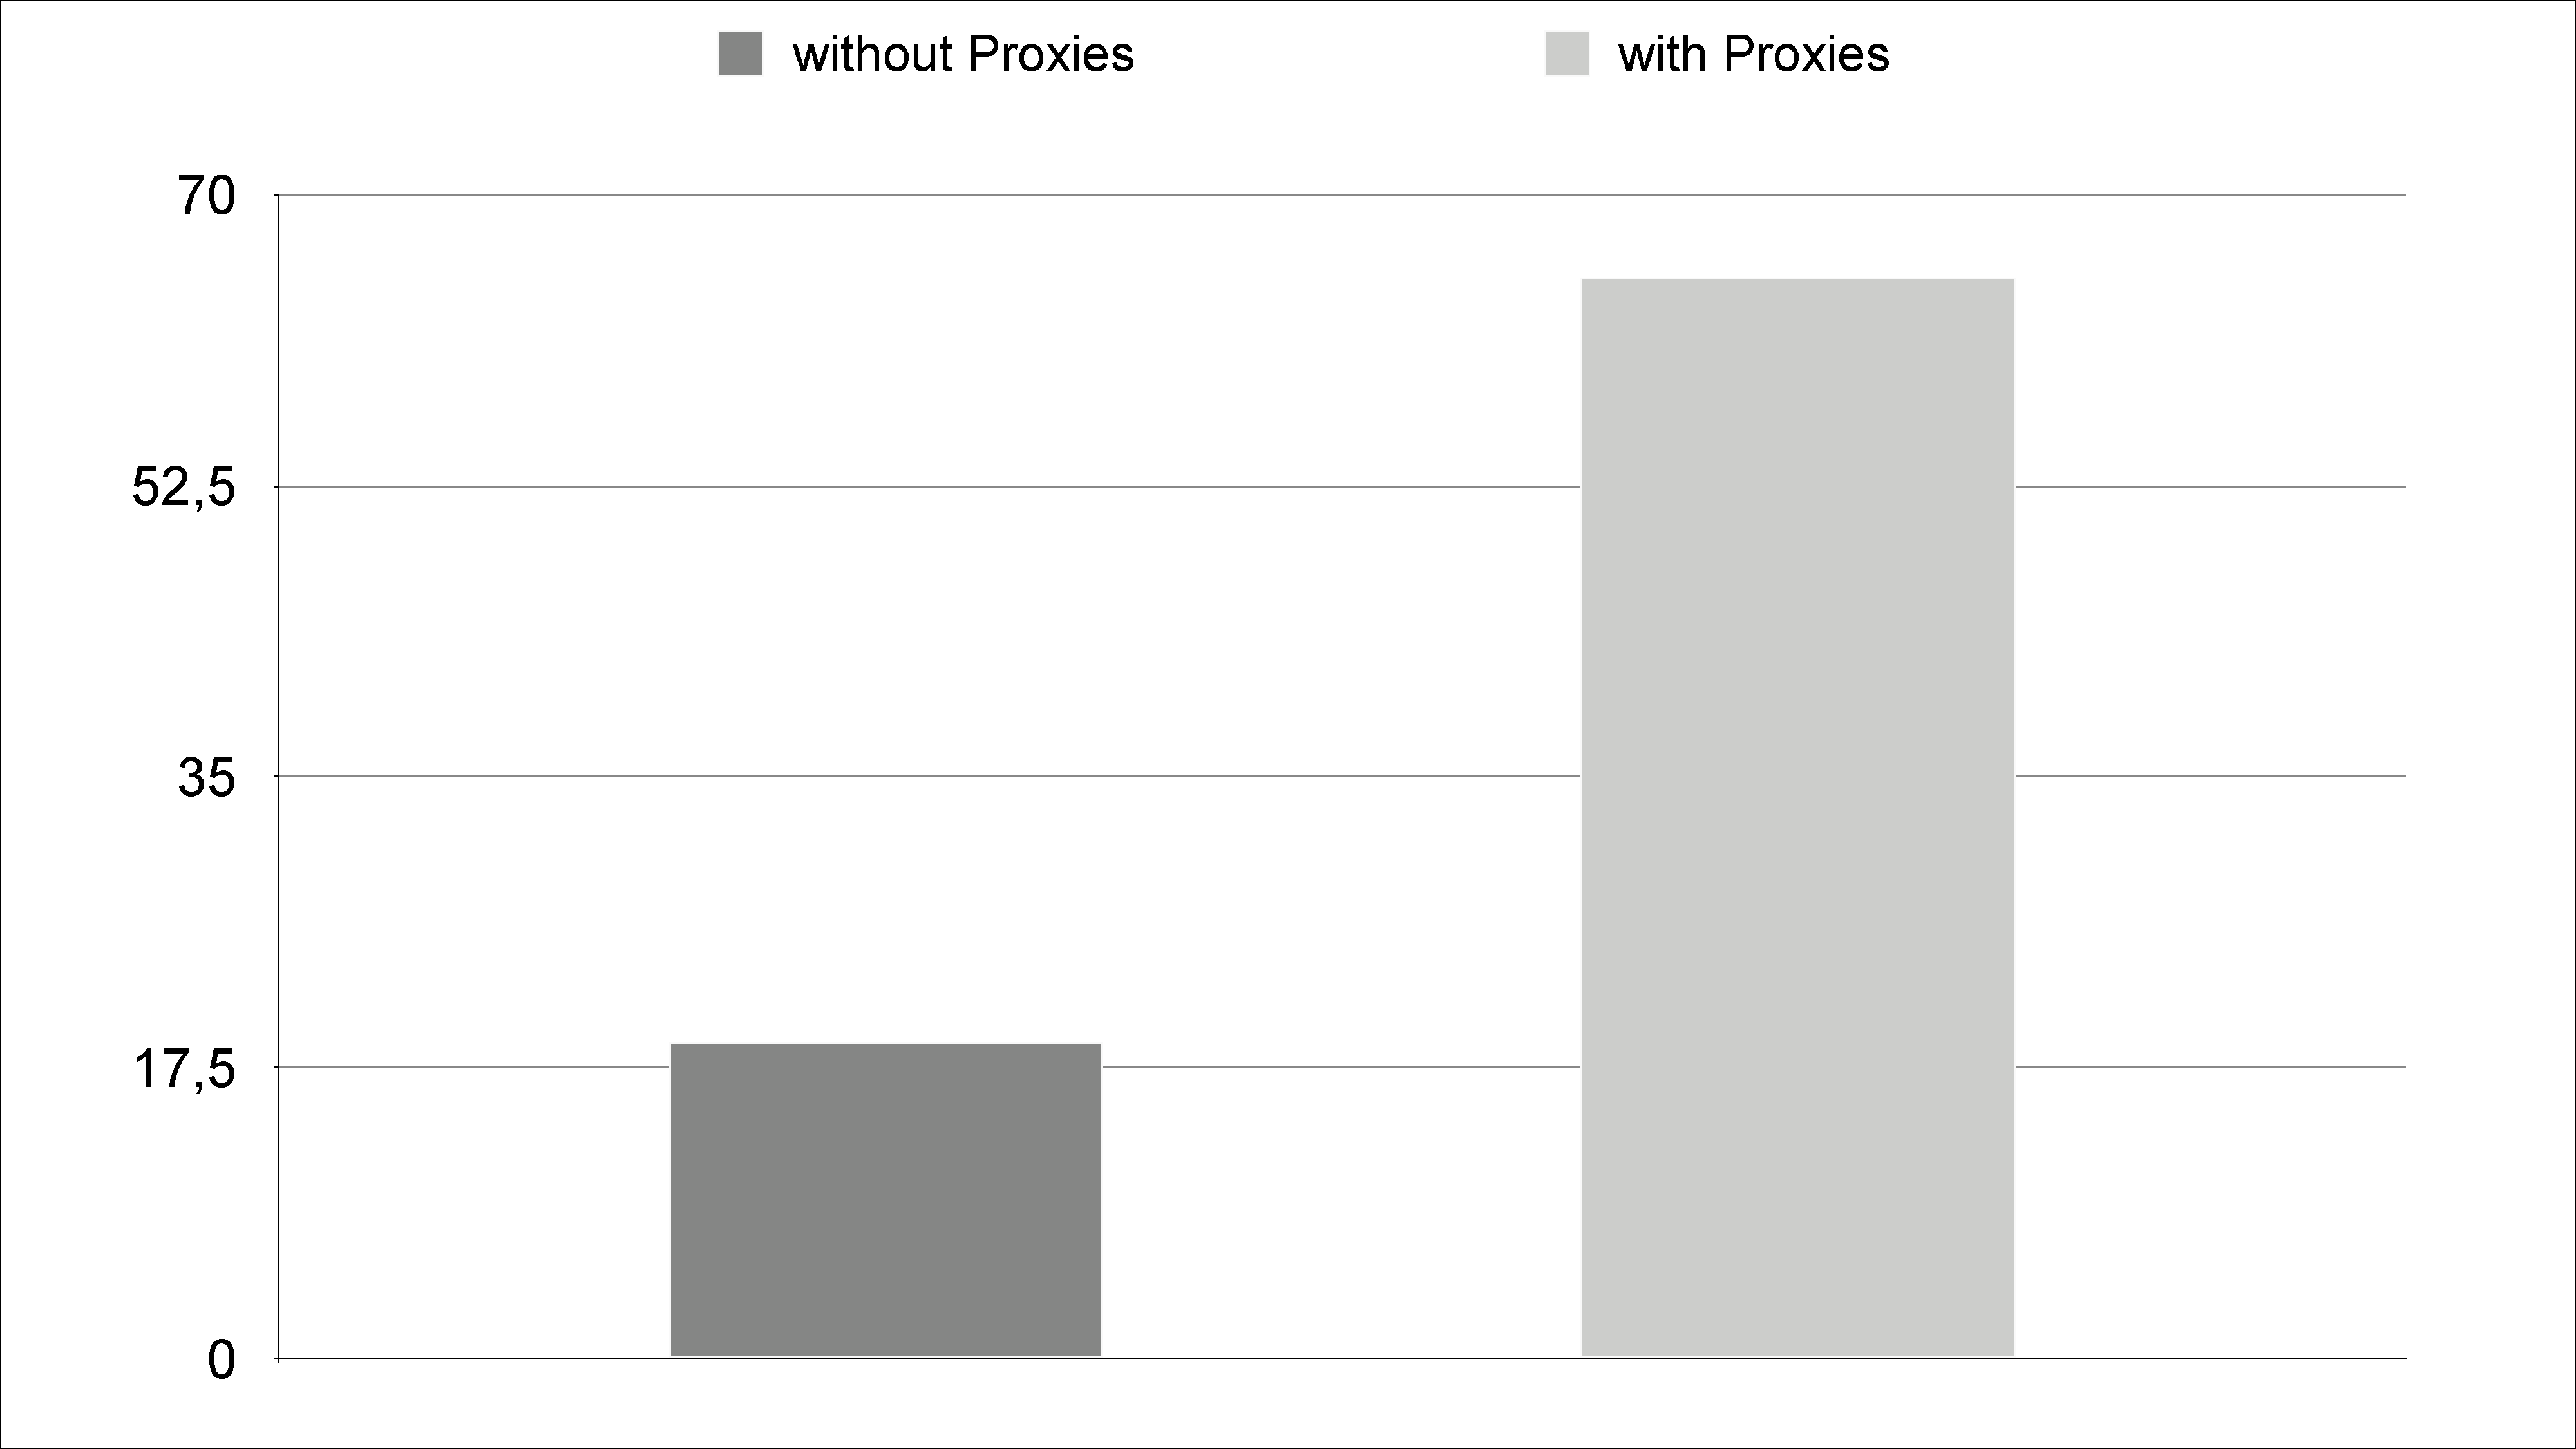
\includegraphics[width=\textwidth]{figures/memoryOverhead.pdf}
    \caption{Memory consumption when starting an empty Lively Kernel environment in megabyte.}
    \label{fig:ExecutionOverhead}
\end{figure}

execution time overhead: for the version-aware references, and the overhead does not increase with the number of versions per object...
\begin{itemize}
    \item common JavaScript language benchmark suites – with vs. without proxies.. see Figure~\ref{fig:ExecutionOverheads}
    \item user interaction benchmarks – with vs. without proxies: starting the lively kernel (including loading a world), opening halos on a morph, opening the world menu, opening the parts bin (/ a workspace / the system code browser), resizing the SCB (programmatically) (?), dragging (programmatically) (?)
\end{itemize}


\begin{figure}[h]
    \centering
    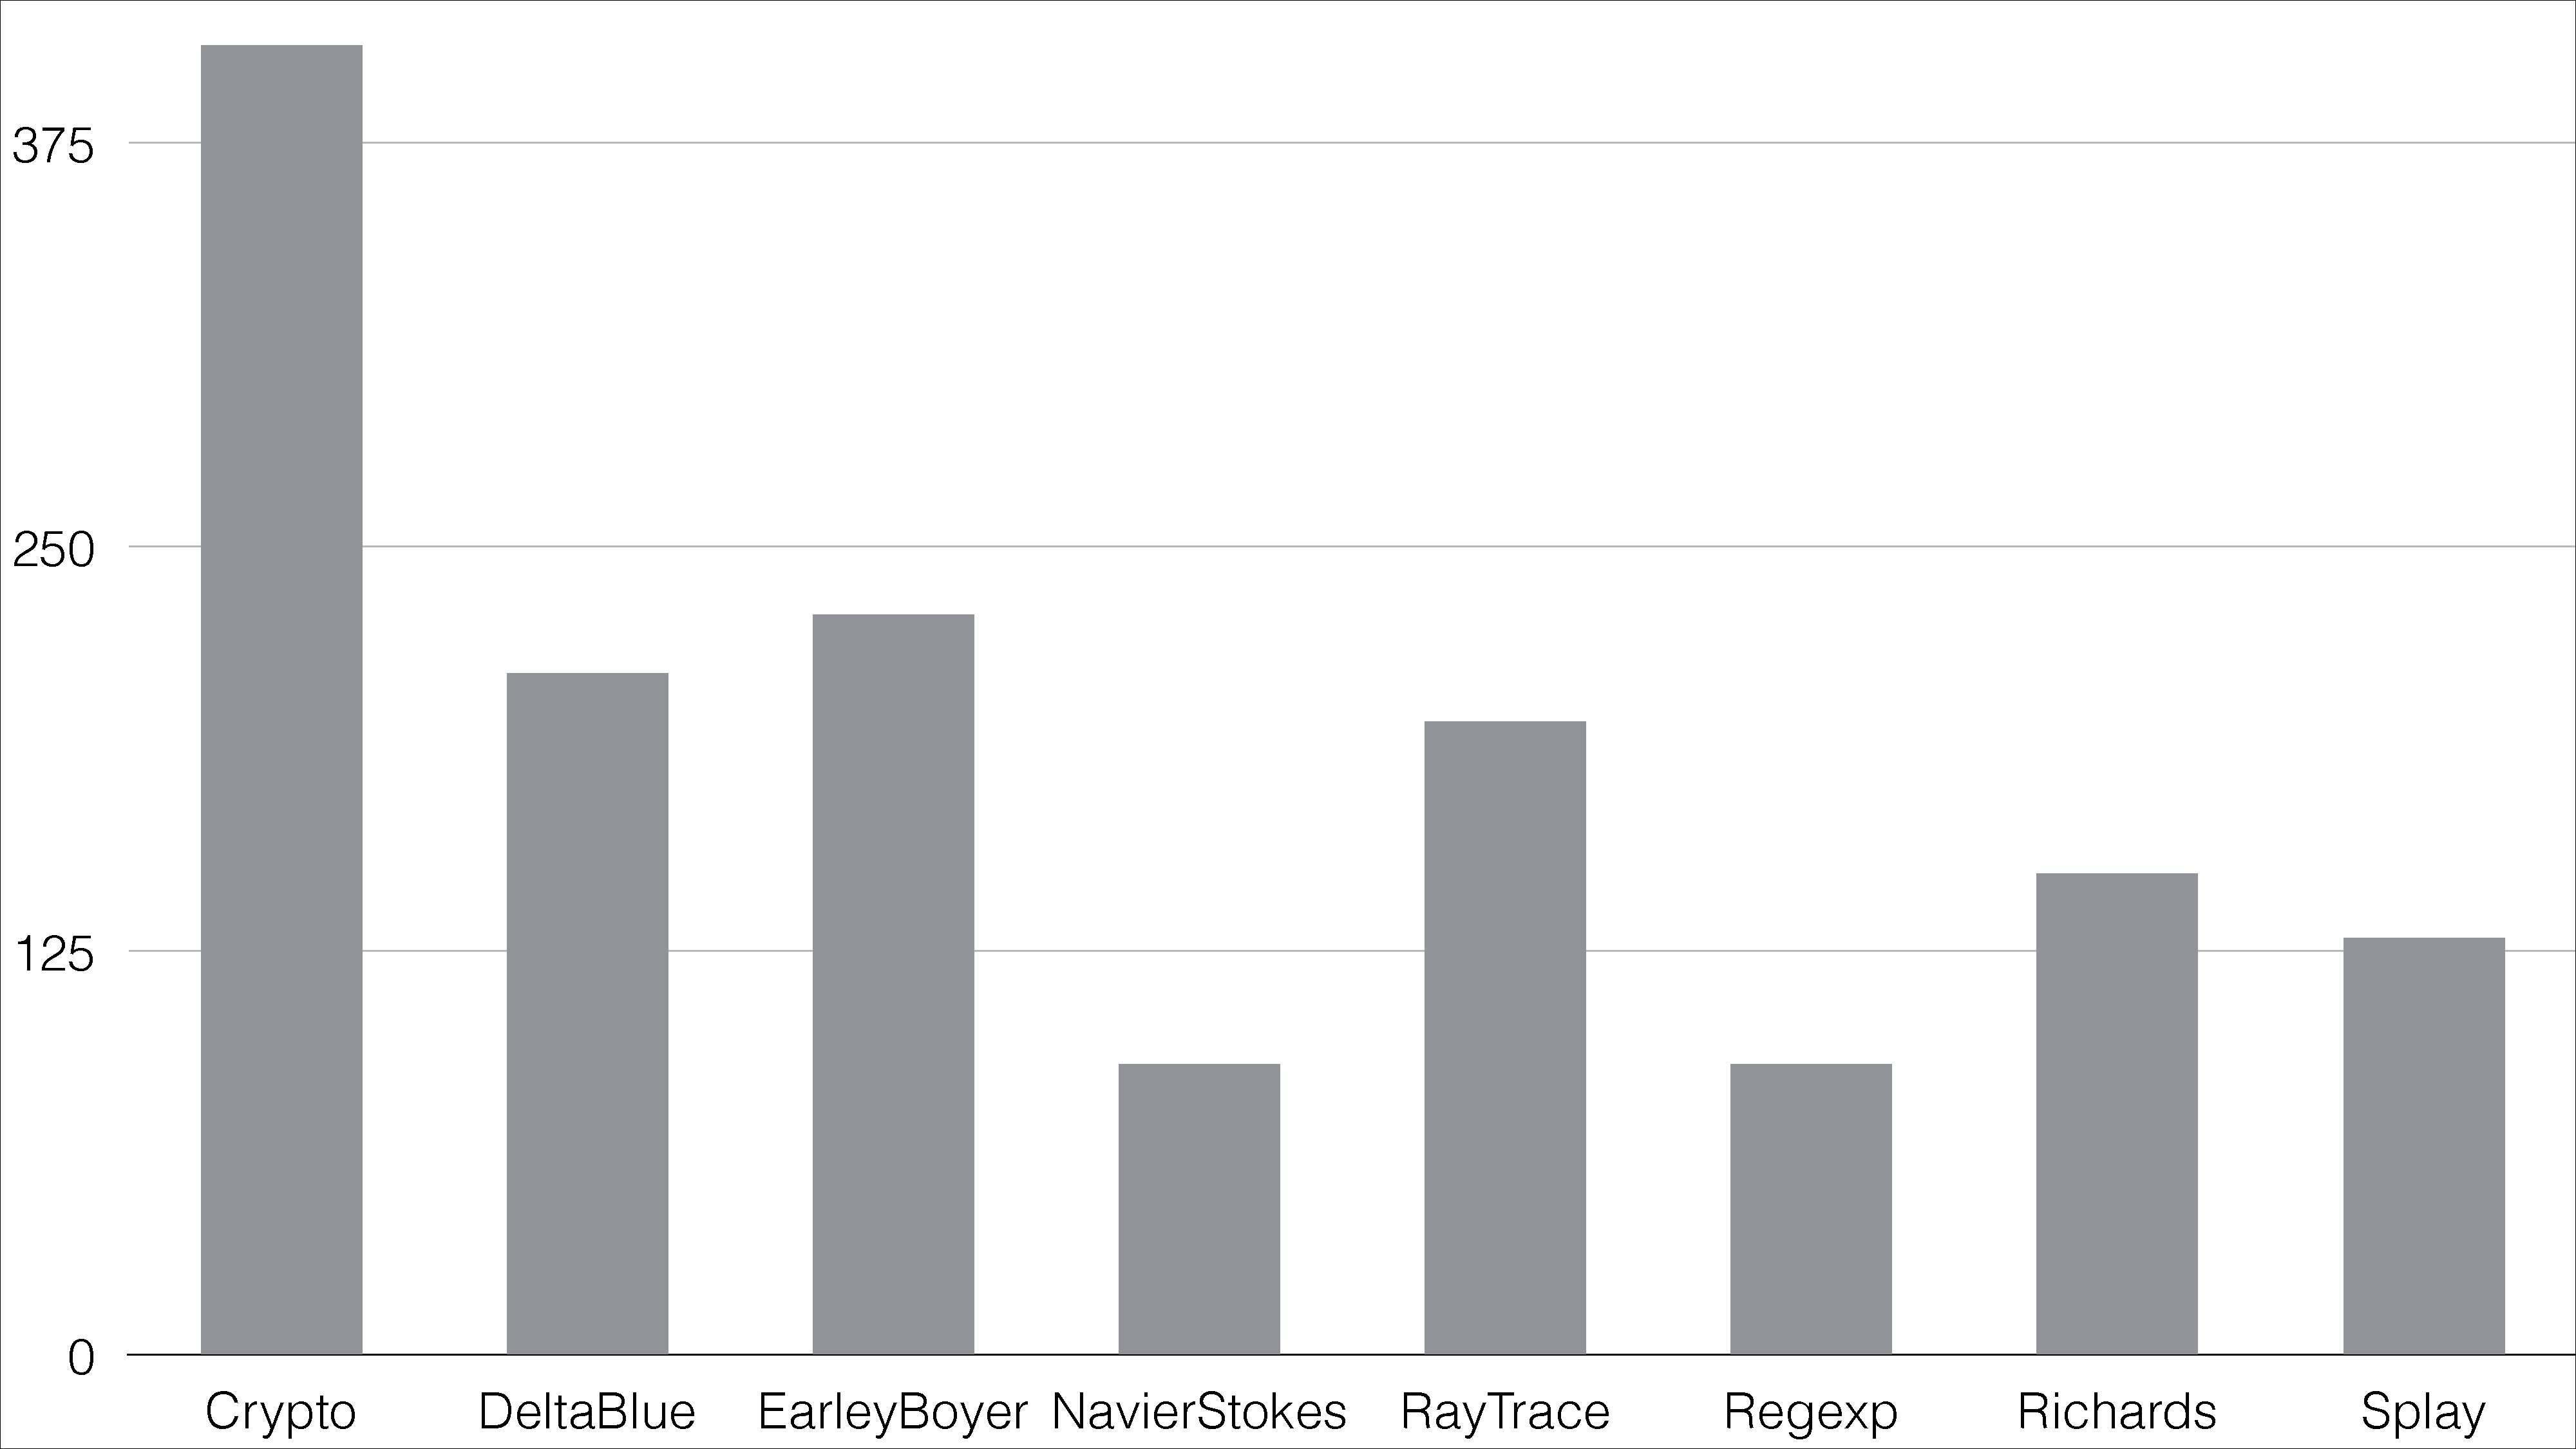
\includegraphics[width=\textwidth]{figures/executionOverhead.pdf}
    \caption{Execution overhead for proxy-based version-aware references in 100\% overhead compared to ordinary JavaScript references.}
    \label{fig:ExecutionOverhead}
\end{figure}



analysis...
maybe some discussion of the execution overhead and numbers on the different layers of the layered implementation cost how much performance: versioning proxy handler > default ES 6 shim proxies > harmony proxies in Chrome..

% This raises questions about the current state of the implementation of the proxies themselves, especially about interference with the v8's JIT compiler, and also indicates more practical implementation strategies.


% say something about how much time it takes to commit and re-establish a version?
\chapter{Related Work} \label{chapter:RELATED_WORK}

\todo{section intro for related work}

\todo{is Johnson and Duggan’s GL programming language related work? (see worlds paper)}
\todo{are Morrisett sub-stores related work? (see worlds papers)}



\section{CoExist}

\cite{Steinert2012COE}
CoExist provides recovery support through continuous versioning in Squeak/Smalltalk.
For each change made to source code, CoExist creates a new version of the system sources, resulting in a fine-grained history of changes.
CoExist then presents this fine-grained history in a timeline and a browser.
For each version, those tools provide diffs, but also test results and a screenshot.
That is, developers do not need to take precautionary actions explicitly during development, but still can easily recover previous development states.
Developers can concentrate on implementing their ideas and as CoExist records a version for each change, there is also no possibility that developers miss a version they need later-on.

Both CoExist and our object versioning record and manage multiple versions of the development state.
They have in common that preserved versions are also part of the program runtime and that versions can be re-established easily.
However, CoExist already records versions continuously on the granularity of changes made by developers and provides much more tool support to find and recover changes from previous versions, which we want to provide for our implementation and the Lively Kernel in the future.
In contrast to CoExist, our system not only preserves code, but also the state of objects and, thus, is primarily intended for programming systems that allow to manipulate objects directly.


\section{Worlds}

Worlds are a language construct to capture and control the scope of side-effects: changes to the state of objects are by default only effective in the world in which the changes occurred.
Worlds are first-class values, to be used to execute statements in a particular world.
A new world can be spawned from an existing world, which establishes a child-parent relationships between the two worlds.
Developers can commit changes contained in a child world to its parent world, thereby extending the scope of the captured side-effects.
For this, the Worlds approach further includes conditions to prevent inconsistencies as result of commits.

In comparison, Worlds provides a language construct to support explicitly experimenting with different states of the runtime, while object versioning provides versions of the runtime intented to be created implicitly and continuously: Our approach does not include extensions to existing programming languages with versions as first-class values and no conditions under which versions of the runtime should be merged into their predecessors.

That said, worlds could, potentially, also be used as a basis for continuous object versioning.
However, out of practical considerations---currently, Worlds, for example, provides no garbage collection and also does not work for all possible JavaScript code---we decided not to build upon worlds, but to implement object versioning as explained in Section~\ref{sec:IMPLEMENTATION}.


\section{Offline Worlds}

Offline Worlds~\cite{Czuchra2012OfW} is an approach to implementing automatic saving of Lively worlds as protection against system failures.
The world is saved automatically in a fixed time interval to be able to re-establish the latest saved version of the world in case of unexpected crashes, or network or server outages.

As only the differences to the last saved version is stored, Offline Worlds would also allow to re-establish other versions than the latest.
However, in contrast to our goals, the Offline Worlds approach aims at preserving the latest state of a Lively world to provide recovery from system failures, while our approach aims to preserve multiple versions of the runtime to provide recovery from inappropriate changes.
Further, Offline Worlds only preserve the state of all graphical objects, whereas our versions also preserve other globally accessible state such as the global system configuration, classes, and state explicitly excluded when serializing graphical objects.
Also, while our approach saves new versions incrementally and resolves to different versions dynamically, Offline Worlds saves and loads versions of the world in a discrete, interruptive step.
While object versioning introduces a constant execution overhead for resolving version-aware references, Offline Worlds stops the world for both saving and loading versions.
For this reason, object versioning seems to be more practical for fine-grained versioning.


\section{Back-in-Time Debugging}

Back-in-time Debuggers~\cite{Lewis2003BIT}, also known as Omniscient Debuggers, allow developers to inspect previous program states and step backwards in the control flow to effectively undo the effects of statements.
For this, approaches are either based on logging or replay: either the debugger records previous states to be able to recreate a particular previous situations, requiring mainly space for all the different states, or the debugger re-executes the program up to a particular previous situation, requiring mainly time to run the program again.
While many logging-based approaches also introduce execution overheads, replay-based approaches need to ensure that the program is re-executed deterministically, which is difficult to ensure when the program relies on state outside of its program runtime as, for example, files or other programs.

Our approach is more related to logging-based back-in-time debugging.
It also allows to re-establish a previous situation through preserving previous states.
However, back-in-time debuggers need to be able to undo the effects of every statement separately, while our system's versioning granularity is arbitrarily and can, for example, correspond to developer interaction with the live system.
In general, back-in-time debuggers support a particular development task---debugging--- and, thus, are also often only active when a program is started in separate debugging mode, while the purpose of object versioning is more comprehensive and we expect it to be active at least during all development tasks, but possibly even be always enabled.

A concrete and particularly related work is Practical Object-oriented Back-in-Time Debugging~\cite{Lienhard2008POB}, a logging-based approach that also preserves the history for each object using alternative references.
As in our approach, these alternative references, called Aliases, are actually also objects, part of the application memory, and contain information about the history and origin of the values stored in objects.
Aliases are, however, never passed around, but new aliases are created for each read or write of an object field or an array and for each reference passed as parameter.
Each of these aliases refers to an actual value, but also to an alias for the value the variable previously referred to---its predecessor---and to the alias that was used to create this new alias from---its origin.
An alias and its origin both refer to the same value, but provide different information as their creation context, which always is a particular method.
That is, the origin link can be used to follow the object's ``flow'' through the program, and, because each alias also records a timestamp when created, the predecessor link can be followed while comparing timestamps to read a value as it were at a particular moment in time.

In comparison to our approach, there is not just one alias object for every mutable object, but potentially many---as many as references to that object, while there is only one version-aware reference.
Further, an alias object has predecessors for every value stored in a variable such as an object field, while our version-aware references hold a subset of the different state the same object had, corresponding to particular discrete versions of the runtime, which may or may not have been commited automatically.
That is, with the presented debugging approach its possible to recreate all states the system was in and also retrace the flow of all values, while our system stores only meaningful versions that, for example, might correspond to developer actions.
Another difference lies in the in the expected usage extent: the alias references are intended to be used only for explicit debugging sessions, while our version-aware reference are intended to be used always, at least completely during all development activities.


\section{Context-oriented Programming}

Context-oriented Programming~\cite{Hirschfeld2008COP} adds dedicated language constructs for dynamic behavior adaptions to object-oriented programs.
Depending on context information, COP allows to enable and disable layers, which contain variations to be executed instead or around methods of the object-oriented base program, at runtime.
Context information can be any information which is computationally accessible.
Different implementation of COP provide different mechansims to scope the activation of layers: often layers can be activated explicitly for a particular scope of the program or globally for the entire runtime.
In ContextJS~\cite{Lincke2011OIC} it is even possible to activate layers only for specific objects.

In comparison to our approach, COP also allows to group changes to the system into layers and which of those sets of changes are active can be changed dynamically.
However, while COP concentrates on behavior variations, our approach recognizes changes to state and behavior.
At the same time, COP supports the composition of multiple layers, while object versioning expects a single specific version to be the current version.
COP further is a language construct that allows to separate heterogeneous cross-cutting concerns, while object versioning is part of the programming system to allow developers to recover previous development states.
However, \cite{Lincke2012SCS} showed that COP can also allow developers to experiment with changes to a system: developers may implement their proposed changes to behavior in layers, not aiming primarily at modularization, but to not change the system permanently and instead be able to recover easily.
Though this requires developers to make experiments explicitly---explicitly creating layers and explicitly moving code from layers back to the base system, once experiments are considered successful and changes expected to be permanent, when developers want to maintain the original modularization of the system.

\section{ChangeBoxes}
ChangeBoxes~\cite{Denker2007EEC}

Class-boxes? \todo{what about Alexandre Bergel's Class-boxes.. and other boxes by the SCG?}



\section{Subject-oriented Programming}
maybe something about David Ungar's Us~\cite{}








\section{Software Transactional Memory}
Software Transactional Memory~\cite{Shavit1995STM}



\section{Scoped Assignments}
Tanter's scoped assignment construct  that enables programmers to control the scope of side effects 




\chapter{Future Work} \label{sec:FUTURE_WORK}

In the future, we want to improve the practicability of our implementation.
Speeding up the proxy-based version-aware references seems most important in this regard.
In addition, we would like to build upon our approach and implementation.
The system should preserve meaningful versions of the runtime automatically and support developers in finding relevant previous state in recovery situations.

\section{Improving the Performance of Our JavaScript Implementation}

Our current implementation makes JavaScript code execution significantly slower and the development tools in Lively considerably less responsiveness, as presented in Section~\todo{ref to 5.2 performance evaluation..}.

Our proxy-based version-aware references select dynamically to which version of an object any access should be delegated.
They also decide dynamically create new versions of an object, when it is changed after having been commited with a version.
Until then, for all reads, our version-aware references delegate to the latest, unchanged version for that object.
With this implementation, creating a new or switching the current version of the runtime happens incrementally instead of in a stop-the-world approach.
At the same time, however, this---the use of version-aware references--introduces a constant runtime overhead.
There will be overhead for incrementally copying objects on writes, when new versions of an object get created, but even for a single active version for the runtime and, thus, for each object, there is the constant overhead of resolving the version-aware references to their current targets.
Thus, when we want to speed-up the execution of JavaScript code and, thereby, also the responsiveness of Lively's tools, we need to reduce the time it takes to resolve a version-aware references, which in the current implementation is done by the proxies.

We use the Direct Proxies that the EcmaScript 6 standard will add to the JavaScript language.
As shown in Section~\todo{ref to 5.2 performance evaluation..}, our specific proxy behavior---delegate to a changing version of an essentially unrelated object---is currently only five times slower than the default behavior---delegate the access unchanged to the proxy's constant target; two orders of magnitude are introduced just by using proxies independent of any version-awareness.
At the time of writing the EcmaScript 6 specification is still only a draft.
We are able to use these proxies already because the Chrome browser implements an earlier, now deprecated specification of the proxies as an experimental feature and because there is a library that provides the currently specified proxies on top of the deprecated style of proxies.
However, given that the proxies are marked as experimental feature and also are currently partly implemented as JavaScript library---on language level instead by the virtual machine---on top of the deprecated variant, it seems reasonable to expect performance gains once the EcmaScript 6 gets finished and implemented by the browser vendors.
Another indicator that proxies could be faster is that equivalent indirections as provided with the proxy handler traps are significantly faster when they are provided manually through ordinary JavaScript functions, also as presented in Section~\todo{ref to 5.2 performance evaluation..}.
This suggests an implementation that is alternative to using the Direct Proxies.
We could still use objects as stand-ins for a multiplicity of versions, but implement the delegation behavior currently provided in proxy traps with ordinary JavaScript functions, which we could use consistently instead of direct object access through further source transformations.
Instead of, for example, \lstinline{anObject.aFunctionProperty()} the system would execute something similar to \lstinline{apply(anObject, get(anObject, aProperty))}.

Besides waiting for faster proxies or not using proxies at all, we could use proxies less deliberately.
Especially not for objects for which we wont have different versions anyways.
One example would be a parser implemented in JavaScript that creates lots of objects while parsing code such as currently used in Lively.
These objects are only necessary during parsing, which often only needs to return a success or a syntax error.
Additionally, given JavaScript single-threaded and cooperative execution in would not even be possible to switch the version during parsing with our current implementation.
So, in this parser example, there wont be multiple versions for any of the objects only created as intermediate results, rendering version-aware reference to such temporary objects irrelevant, while they still impede performance.

\section{Providing Continuous Object Versioning with Recovery Tools}

Our implementation allows to preserve and to re-establish versions of the Lively runtime, but these versions need to be currently created explicitly.
Developers still need to preserve particular versions, which is error-prone and effortful, as explained in Section \todo{refer to code exist section}. Developers might forget to preserve versions, or they underestimate the risk of changes and decide not to preserve a version.
At the same time, it takes effort to assess the risk of upcoming changes, to run appropriate tests to check the current state, and to commit a version.
For these reasons and as suggested by CoExist, we want the system to provide a fine-grained history continuously.
Developers should be able to recover versions that they have not explicitly preserved previously.
This includes that developers also need to be able to find the versions they are looking for.

We could conceivably create versions of the runtime for any change to an object.
However, while that might be technically feasible, developers also need to be able to find and recognize the particular versions they want to recover state from.
Therefore, we propose to preserve versions associated with actions of developers, to allow developers to undo the effects of their actions when they recognize actions did not only improve their programs.
In particular, the system could, for example, automatically preserve a version of the state whenever a developer
\begin{itemize}
    \item manipulates a graphical object directly with one of Lively's halo tools or through drag and drop, or
    \item directly evaluates (``Do-It'') a code snippet, or
    \item saves a script of an object or a method of a class, or
    \item triggers code execution by clicking a button or pressing a key.
\end{itemize}

Besides preserving versions continuously on a granularity helpful to the users, we also want to support developers in finding particular versions of the runtime by adding helpful information to each of the versions.
Versions can be presented in relation to each other in, for example, a timeline.
This way developers could see the order of their actions and for each version of the runtime, which versions preceded and which versions followed.
Such a timeline could also present timestamps for the versions.
Another helpful information would probably be the action that triggered preserving a version such as whether a developer used a halo button or evaluated a code snippet.
This could be supported by recording screenshots or even short screencasts for each version.
A third category of helpful information for a version, besides when and why a version was preserved, could be information on what was changed between two version: which objects have changed and how have they changed.
What source code changed can often be indicated by static information as, for example, a class, its module, and the containing package.
There is, however, less static information for objects.
In case of Livey, for graphical objects, we might be able to present how they relate to the scenegraph of visible objects.
Further, some objects do have explicit names in Lively.
How objects changed between versions can be presented in a diff view for both state and behavior.
Lastly, the system could also provide information on the impact of changes: For each version, we could also preserve results for test cases and benchmarks.

When developers have recovery needs and also find the particular previous version they were looking for, they might want to revisit it for different purposes.
For example, developers might just want to re-establish a particular state of the system to see how an application behaved or looked at that moment.
Similarly, they might want, for example, to try an alternative idea without loosing all versions following the one they are currently revisiting.
That is, they might want to create a branch of changes as an alternative to the main line of versions.
Further, besides moving freely between versions of the runtime as well as creating and deleting lines of history, they also probably will want to recover particular state from particular versions.
Such state could be a particular version of a graphical application part they are working on, but also could be the state of a tool such as a code browser currently opened on a specific source code module.
For this, we want to support developers in copying particular state up to whole objects from one version of the runtime to another.

All in all, this tool support for recovery should allow developers to find and re-establish versions, to create and delete lines of histories, and to diff and merge changes from one version of the system to another.

\chapter{Conclusion} \label{chapter:CONCLUSION}

% Approach

% Significance, Practical applications

% Future work
In the future, 

% Summary sentence
Nevertheless,


% \chapter{Introduction}

% Here goes the foo.\todo{cite here}
% I will talk about what an \ac{api} is in this section.
% Normally, there are different \acp{api}. Not to forget,
% anything can be an \ac{api}. And full: \acf{api}.

\printbibliography
\clearpage
% \appendix
% %% ggf:
\part{Appendix}
\label{part:appendix}

% \chapter{First Unimportant stuff.} \label{cha:first-unimp-stuff}

% \blindtext

%%% Local Variables: 
%%% mode: latex
%%% End: 

\backmatter
\markboth{}\relax
\defaultstatement
\end{document}
%%% Local Variables:
%%% mode: latex
%%% TeX-master: t
%%% End:
